\documentclass[a4paper, 12pt]{article}
\usepackage[margin=24mm]{geometry}
\usepackage{float}
\usepackage{titling}
\usepackage{graphicx}
\usepackage{caption}
\usepackage{subcaption}
\usepackage[hidelinks]{hyperref}
\usepackage[toc,page]{appendix}
\usepackage{multirow}
%
%\geometry{bindingoffset=35mm}

\providecommand{\keywords}[1]{\textbf{\textit{Keywords ---}} #1}

\begin{document}
\thispagestyle{empty}
\setcounter{page}{0}
\begin{abstract}\textbf{\emph{
Contrary to popular belief, skydiving is a competitive and technical sport, requiring careful control of body position in order to not only remain stable, but also to move around the sky in free-fall. A popular discipline in competitive skydiving is formation skydiving, where a group of skydivers form set shapes with their bodies whilst in free-fall. This Report proposes a software tool to be written; able to automatically judge  formation skydiving footage. This will be done detecting the pose of each skydiver in the formation individually; this information will then be used to find the overall shape of the formation. This tool will combine and extend well established computer vision methods such as Active Shape Models, skeletonisation. The ultimate goal is to remove the need for manual competition judging, switching to a fully automated system.
}}\end{abstract}
\clearpage
%
\section{Background}
	\subsection{Formation Skydiving}
Skydiving is a competitive and technical sport, requiring careful control of body position in order to move around the sky in a controlled manner whilst in free-fall.\\
A popular discipline in the sport is formation skydiving (FS). This involves multiple skydivers forming set shapes with their bodies, in order to score as many points as possible.
		\subsubsection{Rules}
		A point is awarded for each successful formation in a sequence \textbf{\emph{(see figure \ref{fig:fs_dive_pool})}}. A successful formation is defined only by the correct hands of each skydiver holding the correct grips on the other skydivers \textbf{\emph{(see figure \ref{fig:grips})}}, and not by the orientation of the skydivers themselves.
%
\begin{figure}[H]
	\centering
	\includegraphics[width=0.9\linewidth]{grips.png}
	\caption{Diagram showing all of the available grips on a formation skydiving suit.}
	\label{fig:grips}
\end{figure}
%
\noindent In 4 person FS (4-way FS) each skydiver has a specific slot in the formation. This is the position that they will always take when making each formation. This is done in such a way that the amount of movement required for each skydiver when transitioning between formations is minimised. The four slots in 4-way FS are known as Point, Tail, Outside Center (OC) and Inside Center (IC). 
%
	\subsubsection{Training Practices}
In order for the team to create formations in the sky, it is important that they practice the skydive multiple times on the ground. This is known as "dirt diving" and is often done using partially triangular wheeled platforms that each skydiver lays on, known as "creepers"  \textbf{\emph{(see figures \ref{fig:creepers} and \ref{fig:creepers_use})}}.
\begin{figure}[H]
	\centering
	\begin{subfigure}{.5\textwidth}
		\centering
		\includegraphics[width=0.9\linewidth]{creepers.jpg}
		\caption{FS practice platforms "creepers"}
		\label{fig:creepers}
	\end{subfigure}%
	\begin{subfigure}{.5\textwidth}
		\centering
		\includegraphics[width=0.9\linewidth]{creepers_use.jpg}
		\caption{"Creepers" in use while "dirt diving" a "Donut" formation}
		\label{fig:creepers_use}
	\end{subfigure}
	\caption{Images reproduced from \url{www.skydivespaceland.com/blog/images/creepers2.jpg} and \url{www.skydiveaz.com/images/old-images/creepers.jpg}}
\end{figure}
%
\noindent Another way that FS teams train is to use a vertical (indoor skydiving) wind tunnel. A fan is mounted at the bottom of the tunnel creating a strong wind that the skydivers can float on; simulating the environment of a regular skydive, but in a much more controlled environment \textbf{\emph{(see figure \ref{fig:sample_tunnel})}}.
	\subsection{Project Brief}
The original focus of the project was to analyse video of dirt diving and identify which formations have been performed. The focus has been changed slightly, and is now to analyse footage of formation skydiving in a vertical wind tunnel. This change is largely due to the fact that the body position of a skydiver free-fall is much more similar to their body position in a wind tunnel, than when dirt diving. Another benefit of analysing footage taken in a wind tunnel is that the camera is mounted above the formation, remaining static \textbf{\emph{(see figure \ref{fig:sample_tunnel})}}. This allows the skydivers to much more easily be separated from the background via background subtraction\cite{Piccardi}. The set of formations that will be analysed are the BPA rookie class of formations known as 'randoms'. The software must be able to recognise all 16 of the randoms \textbf{\emph{(see figure \ref{fig:fs_dive_pool})}}.
%
\begin{figure}[H]
	\centering
	\includegraphics[width=\linewidth]{FS_All.png}
	\caption{All 16 BPA rookie class FS 'randoms' formations, with their names. The colours for each slot are: Point red, OC green, IC blue, Tail yellow.\\
	Reproduced from \url{http://www.teamsatori.co.uk/New\%204W\%20Random\%20Dive\%20pool.pdf}}
	\label{fig:fs_dive_pool}
\end{figure}
%
\begin{figure}[H]
	\centering
	\begin{subfigure}{.5\textwidth}
		\centering
		\includegraphics[width=0.9\linewidth]{Tunnel_Star.png}
	\end{subfigure}%
	\begin{subfigure}{.5\textwidth}
		\centering
		\includegraphics[width=0.9\linewidth]{Tunnel_Sidebody.png}
	\end{subfigure}\\
	\begin{subfigure}{.5\textwidth}
		\centering
		\includegraphics[width=0.9\linewidth]{Tunnel_Phalanx.png}
	\end{subfigure}%
	\begin{subfigure}{.5\textwidth}
		\centering
		\includegraphics[width=0.9\linewidth]{Tunnel_Donut.png}
	\end{subfigure}%
	\caption{Sample FS formations performed in a wind tunnel, with their names.\\
	Images reproduced from International Bodyflight Association, \url{www.youtube.com/watch?v=Y2B4S3lGf54&list=LLsEkKn0qzIHSGefmSGT_4og}. }
	\label{fig:sample_tunnel}
\end{figure}
%
\noindent An image of a skydiver in an FS body position can be simplified to a set of line segments between 11 key points; one for the waist, neck, head, left and right hands, elbows, knees and feet \textbf{\emph{(see figure \ref{fig:stick_model_fitted})}}.
%
\begin{figure}[H]
	\centering
	\includegraphics[width=\linewidth]{stick_model_fitted.png}
	\caption{Diagram showing how an image of a skydiver can be simplified to a set of line segments between 11 points.}
	\label{fig:stick_model_fitted}
\end{figure}
%
\noindent In order to complete this project C++ will be used, making use of the open source computer vision library OpenCV 3.0\cite{\cite{OpenCV}} in order to reduce the time required to perform standard tasks, such as loading an image file, or receiving a video feed.
If a graphical user interface (GUI) were to be implemented, the open source GUI library Qt 5.3\cite{Qt} would be used.
These libraries are platform independent; this should ensure that the program is not tied to any single operating system.
%

\section{Literature Report}
%
Due to the specialist nature of the project, relevant existing literature is somewhat limited.
However, there does exist relevant literature on various methods for human posture recognition.

\subsection{Posture Detection}
%
Human pose detection can be a difficult problem to tackle; many factors contribute towards this, such as shadows, occlusions, complicated backgrounds and noisy source images.\\
There are many different proposed methods to tackle the task of human posture detection; over a wide variety of technologies. Some methods use depth cues extracted from 3d scanner information, such as \cite{kinect_IR} which uses a Microsoft Kinect to detect the human body. Other methods are designed to work with video\cite{video}, creating a 3d estimation of human pose in order to detect people. A common goal is to try to detect the pose of a person from a single static image. There are a variety of ways of doing this such as, using a model-based method, where an explicit pose model must be specified, often requiring complicated 3d modelling and rendering\cite{model-based}. Another method used relies on texture cues in order to perform "Parts-based" object detection\cite{monocular_still_images}, this method neither uses an explicit model, or pre-labelled data.\\
However, the method that is deemed to most fit goal of recognising the pose of a skydiver is an adaptive method, such as Active Shape Models. Active Shape Models are more often used in facial feature detection\cite{cootes}\cite{face_recognition}; given that it only relies on a set of simple points, labelled from a set of training images it should be ideal for the task at hand.
%
\subsection{Active Shape Models}
Active Shape Models are statistical shape models that are able iteratively deform in order to fit a given example image. They can also be used to characterise the ways in which a set of points in an image can move. Using principal component analysis\cite{icl_pca}, it is possible to find a minimal set of feature variables which control the overall shape of an object. Varying these enables every possible permutation of the set of image points to be found.\\
In order for this to be done, a training set of points must be collected by hand from images similar to those that will be analysed. This This training set of points forms the initial point matrix.
%
\begin{figure}[H]
	\centering
	\includegraphics[width=.5\linewidth]{shape_matrix.png}
	\caption{Initial point matrix. Each row corresponds to a different image (blue). Pairs of columns contain coordinates of the same point across each of the images (red).}
	\label{fig:shape_matrix}
\end{figure}
%
\noindent The iterative algorithm generalised procrustes analysis (GPA) is then used to optimally rotate, scale, and translate the points from each image. The goal of this is to have the points from each image match as closely as possible when superimposed on each other \textbf{\emph{(see figure \ref{fig:procrastes})}}.
%
\begin{figure}[H]
	\centering
	\includegraphics[width=\linewidth]{generalised_procrastes_ananlysis.png}
	\caption{Performing generalised procrustes analysis on three shapes.}
	\label{fig:procrastes}
\end{figure}
%
\noindent A shape matrix can be created using the same format as the initial point matrix, but containing the coordinates of the aligned image points.
Finally, principal component analysis is used to reduce the dimensions of the shape matrix. This is done by finding the eigenvalues and eigenvectors of the covariance matrix. A more in depth explanation can be found at \cite{icl_pca}.\\
\\
Using this method it is possible to find weather a skeleton of a skydiver is viable or not. This is done by creating the initial point matrix from a set of images of a skydiver in a variety of FS body positions. The resulting active shape model will contain information defining how a skydiver's body position can change. A set of test points that make up the skydiver's skeleton \textbf{\emph{(see figure \ref{fig:stick_model_fitted})}} can then be compared to this model to find if the skeleton is possible or not. This allows the skeleton to be recalculated, should it be found to be impossible.
%
%
\section{Proposed Final Design}
%
The proposed final design will take the form of a command line tool. It will take the path to a video of formation skydiving to be analysed as an argument. It's output will be a similar video file, but with an overlay showing which (if any) formations have been made at each stage in the video. It will also highlight the skeletons of the skydivers in different colours in order to show which slot in the formation they are flying. The skeletons will take the same colours as in \textbf{\emph{figure \ref{fig:fs_dive_pool}}}. Time permitting, a GUI may be implemented for the command line tool in order to make the software more user friendly.\\
\\
Given that the project is entirely software based, additional support towards the project should not be necessary.
\subsection{Flow Chart}
%
\begin{figure}[H]
	\centering
	\includegraphics[width=\linewidth]{flow_chart.png}
	\caption{Flowchart showing overall functionality of proposed final design. Items shown in green have been completed. Items inside the red box are to be executed only once, and their results saved for later use.}
	\label{fig:flowchart}
\end{figure}
%
%
\section{Completed Work}
	\subsection{Data Collection}
	Software has been written that handles collection of data for the initial point 			matrix to be used to create the point distribution model. In order to speed up data collection, the program displays an image of a skydiver and asks the user to left click on different parts of the skydiver's body. The user can undo the last point by right clicking. Once all the points for the image are recorded, they are written to an output file and form the next row of the initial point matrix. Another image is then shown and the process repeats. This is a console based application and takes the file path of an image list as its only input \textbf{\emph{(see figure \ref{fig:data_collection})}}. This image list is stored in an XML file, as OpenCV natively supports input and output to XML files. For each image, the program adds another row to the initial point matrix \textbf{\emph{(see figure \ref{fig:shape_matrix})}}. Currently only 10 images have been used to create the initial point matrix, but this number will be increased before it is used to create the point distribution model.
%
\begin{figure}[H]
	\centering
	\includegraphics[width=\linewidth]{data_collection.png}
	\caption{Data labelling program. Screenshot taken once all the required points of the image had been clicked on.}
	\label{fig:data_collection}
\end{figure}
%
\begin{figure}[H]
	\centering
	\includegraphics[width=\linewidth]{initial_matrix.png}
	\caption{Matrix created when the program is supplied with a sample image list with 10 images in it.}
	\label{fig:initial_matrix}
\end{figure}
%
	\subsection{Skeletonisation}
	Software has been written that creates a minimal, connected, 1 pixel thick skeleton from a binary mask. The function uses a medial axis transformation based method \cite{skeletonisation}  to create the skeleton and the Ramer--–Douglas–--Peucker\cite{Ramer}\cite{Douglas_Peucker} (RDP) algorithm to minimise it.
%
\subsubsection{Skeletonisation Algorithm}
        \begin{enumerate}
   		\item Find all boundary pixels (edge of the binary mask) using a binary laplacian mask\cite{binary_laplacian}. For each boundary pixel do the following:
        \item{Test pixels neighbours
        %
\begin{table}[H]
\centering
\begin{tabular}{llll}
\cline{1-3}
\multicolumn{1}{|l|}{p8} & \multicolumn{1}{l|}{p1} & \multicolumn{1}{l|}{p2} & y \\ \cline{1-3}
\multicolumn{1}{|l|}{p7} & \multicolumn{1}{l|}{p0} & \multicolumn{1}{l|}{p3} &  \\ \cline{1-3}
\multicolumn{1}{|l|}{p6} & \multicolumn{1}{l|}{p5} & \multicolumn{1}{l|}{p4} & $\downarrow$ \\ \cline{1-3}
x &  & $\rightarrow$ & 
\end{tabular}
\end{table}}
%
        \item Count Np0, number of non-zero neighbours of p0.
        \item Count Tp0, number of 0-1 transitions in sequence p1, p2, ..., p8.
        \item Check the initial conditions; mark for deletion any point that satisfies them all.\\
        Initial conditions:
        \begin{itemize}
         \item $cA:     2 <= Np0 <= 6$
         \item $cB:     Tp1 = 1$
         \item $cC:     p1 . p3 . p5 = 0$
         \item $cD:     p3 . p5 . p7 = 0$
         \end{itemize} 
         
        \item Delete any points marked for deletion.
        \item For each remaining boundary pixel, recalculate Np0 and Tp0, then check secondary conditions; marking for deletion any point that satisfies them all:\\
Secondary conditions:
        \begin{itemize}
        \item $cA:     2 <= Np0 <= 6$
        \item $cB:     Tp1 = 1$
        \item $cC\_:    p1 . p3 . p7 = 0$
        \item $cD\_:    p1 . p5 . p7 = 0$
        \end{itemize}
        \item Delete any points marked for deletion.
        \end{enumerate}
%
Repeat process until no points are deleted.\\
For more a more in depth explanation of the algorithm, see \cite{skeletonisation}.\\
\\
Initially a simpler algorithm\cite{skeletonisation_simple} was used in order to create the skeleton using morphological operations to perform thinning. However, this algorithm did not ensure that the skeleton created was minimal or connected, and was therefore insufficient.
\begin{figure}[H]
	\centering
	\includegraphics[width=\linewidth]{skel_simple.jpg}
	\caption{Result of using the morphological thinning algorithm on the binary image shown in \textbf{\emph{figure \ref{fig:skel_src_mask}}}.}
	\label{fig:skel_simple}
\end{figure}
\subsubsection{Skeleton Simplification Algorithm}
	The RDP algorithm is designed to simplify a curve, while still maintaining its overall shape. A curve can be thought of as a collection of linked line segments, with each line segment stretching between two consecutive points on the curve. The basic principle of the algorithm is to reduce the number of line segments in a curve; creating a similar, but simplified curve. The algorithm is initially given an ordered array of all the points in the curve. The algorithm is also given the variable $\epsilon$; this defines the degree to which the curve should be simplified and represents a minimum distance between line segments on the curve. It marks the start and end points of the curve as the first line segment (L), and then finds the point furthest from this initial line segment. If the distance from this point to the line segment (d) is less than $\epsilon$ then it is marked for removal. If the point is further than $\epsilon$ then it is kept and the algorithm recursively called with this point as the new end point. In this way the algorithm is able to remove every point that is closer than $\epsilon$ to the line segment that joins its neighbours.
%
\begin{figure}[H]
	\centering
  	\includegraphics[width=\textwidth]{douglas_peucker.png}
  	\caption{Diagram showing the RDP algorithm working on a curve. 0 being the initial curve to be simplified, and 4 being the fourth result the algorithm. Red arrows show points marked for deletion, green arrows show points to be kept\\
  	Modified from \url{http://upload.wikimedia.org/wikipedia/commons/9/91/Douglas_Peucker.png}.}
  	\label{fig:douglas_peucker}
\end{figure}
%
\noindent The RDP algorithm is used to reduce the number of points in the skeleton, simplifying it; however, it is only able to simplify curves with no bifurcations. This proves to be a problem when trying to simplify a skeleton produced by the skeltonisation algorithm, as it will always have bifurcations at the waist and neck. It may also also produce erroneous bifurcations at other points on the skeleton. These bifurcations can be seen in \textbf{\emph{figure \ref{fig:skel}}}.\\
The location of these bifurcations can be detected by applying a modified version of condition $cB$ from the skeletonisation algorithm. Tp0 is calculated in the same way, by looking at the number of 0-1 transitions in the sequence p1, p2, ... , p8.
%
\begin{table}[h]
\centering
\begin{tabular}{llll}
\cline{1-3}
\multicolumn{1}{|l|}{p8} & \multicolumn{1}{l|}{p1} & \multicolumn{1}{l|}{p2} & y \\ \cline{1-3}
\multicolumn{1}{|l|}{p7} & \multicolumn{1}{l|}{p0} & \multicolumn{1}{l|}{p3} &  \\ \cline{1-3}
\multicolumn{1}{|l|}{p6} & \multicolumn{1}{l|}{p5} & \multicolumn{1}{l|}{p4} & $\downarrow$ \\ \cline{1-3}
x &  & $\rightarrow$ & 
\end{tabular}
\end{table}
%
\\If $Tp0 > 2$ then a bifurcation is present at p0.
This is always true, as the skeletonisation algorithm ensures that the skeleton is a single pixel thick 8-connected component.\\
Once the location                               of every bifurcation is found, the skeleton can be split into separate curves, by removing the bifurcation point. The RDP algorithm is then run on each of these curves independently. The simplified curves can then be recombined to form a simplified skeleton. At this point it is also possible the remove the false skeleton sections created by the skeletonisation algorithm forming erroneous bifurcations. The simplest way to do this is to delete any simplified skeleton section that is shorter than a given length. This works as the false skeleton sections tend to be shorter than the correct ones. A more reliable method for detecting false skeleton sections could be used in the final design.
\begin{figure}[H]
	\centering
	\begin{subfigure}{.5\textwidth}
  		\centering
  		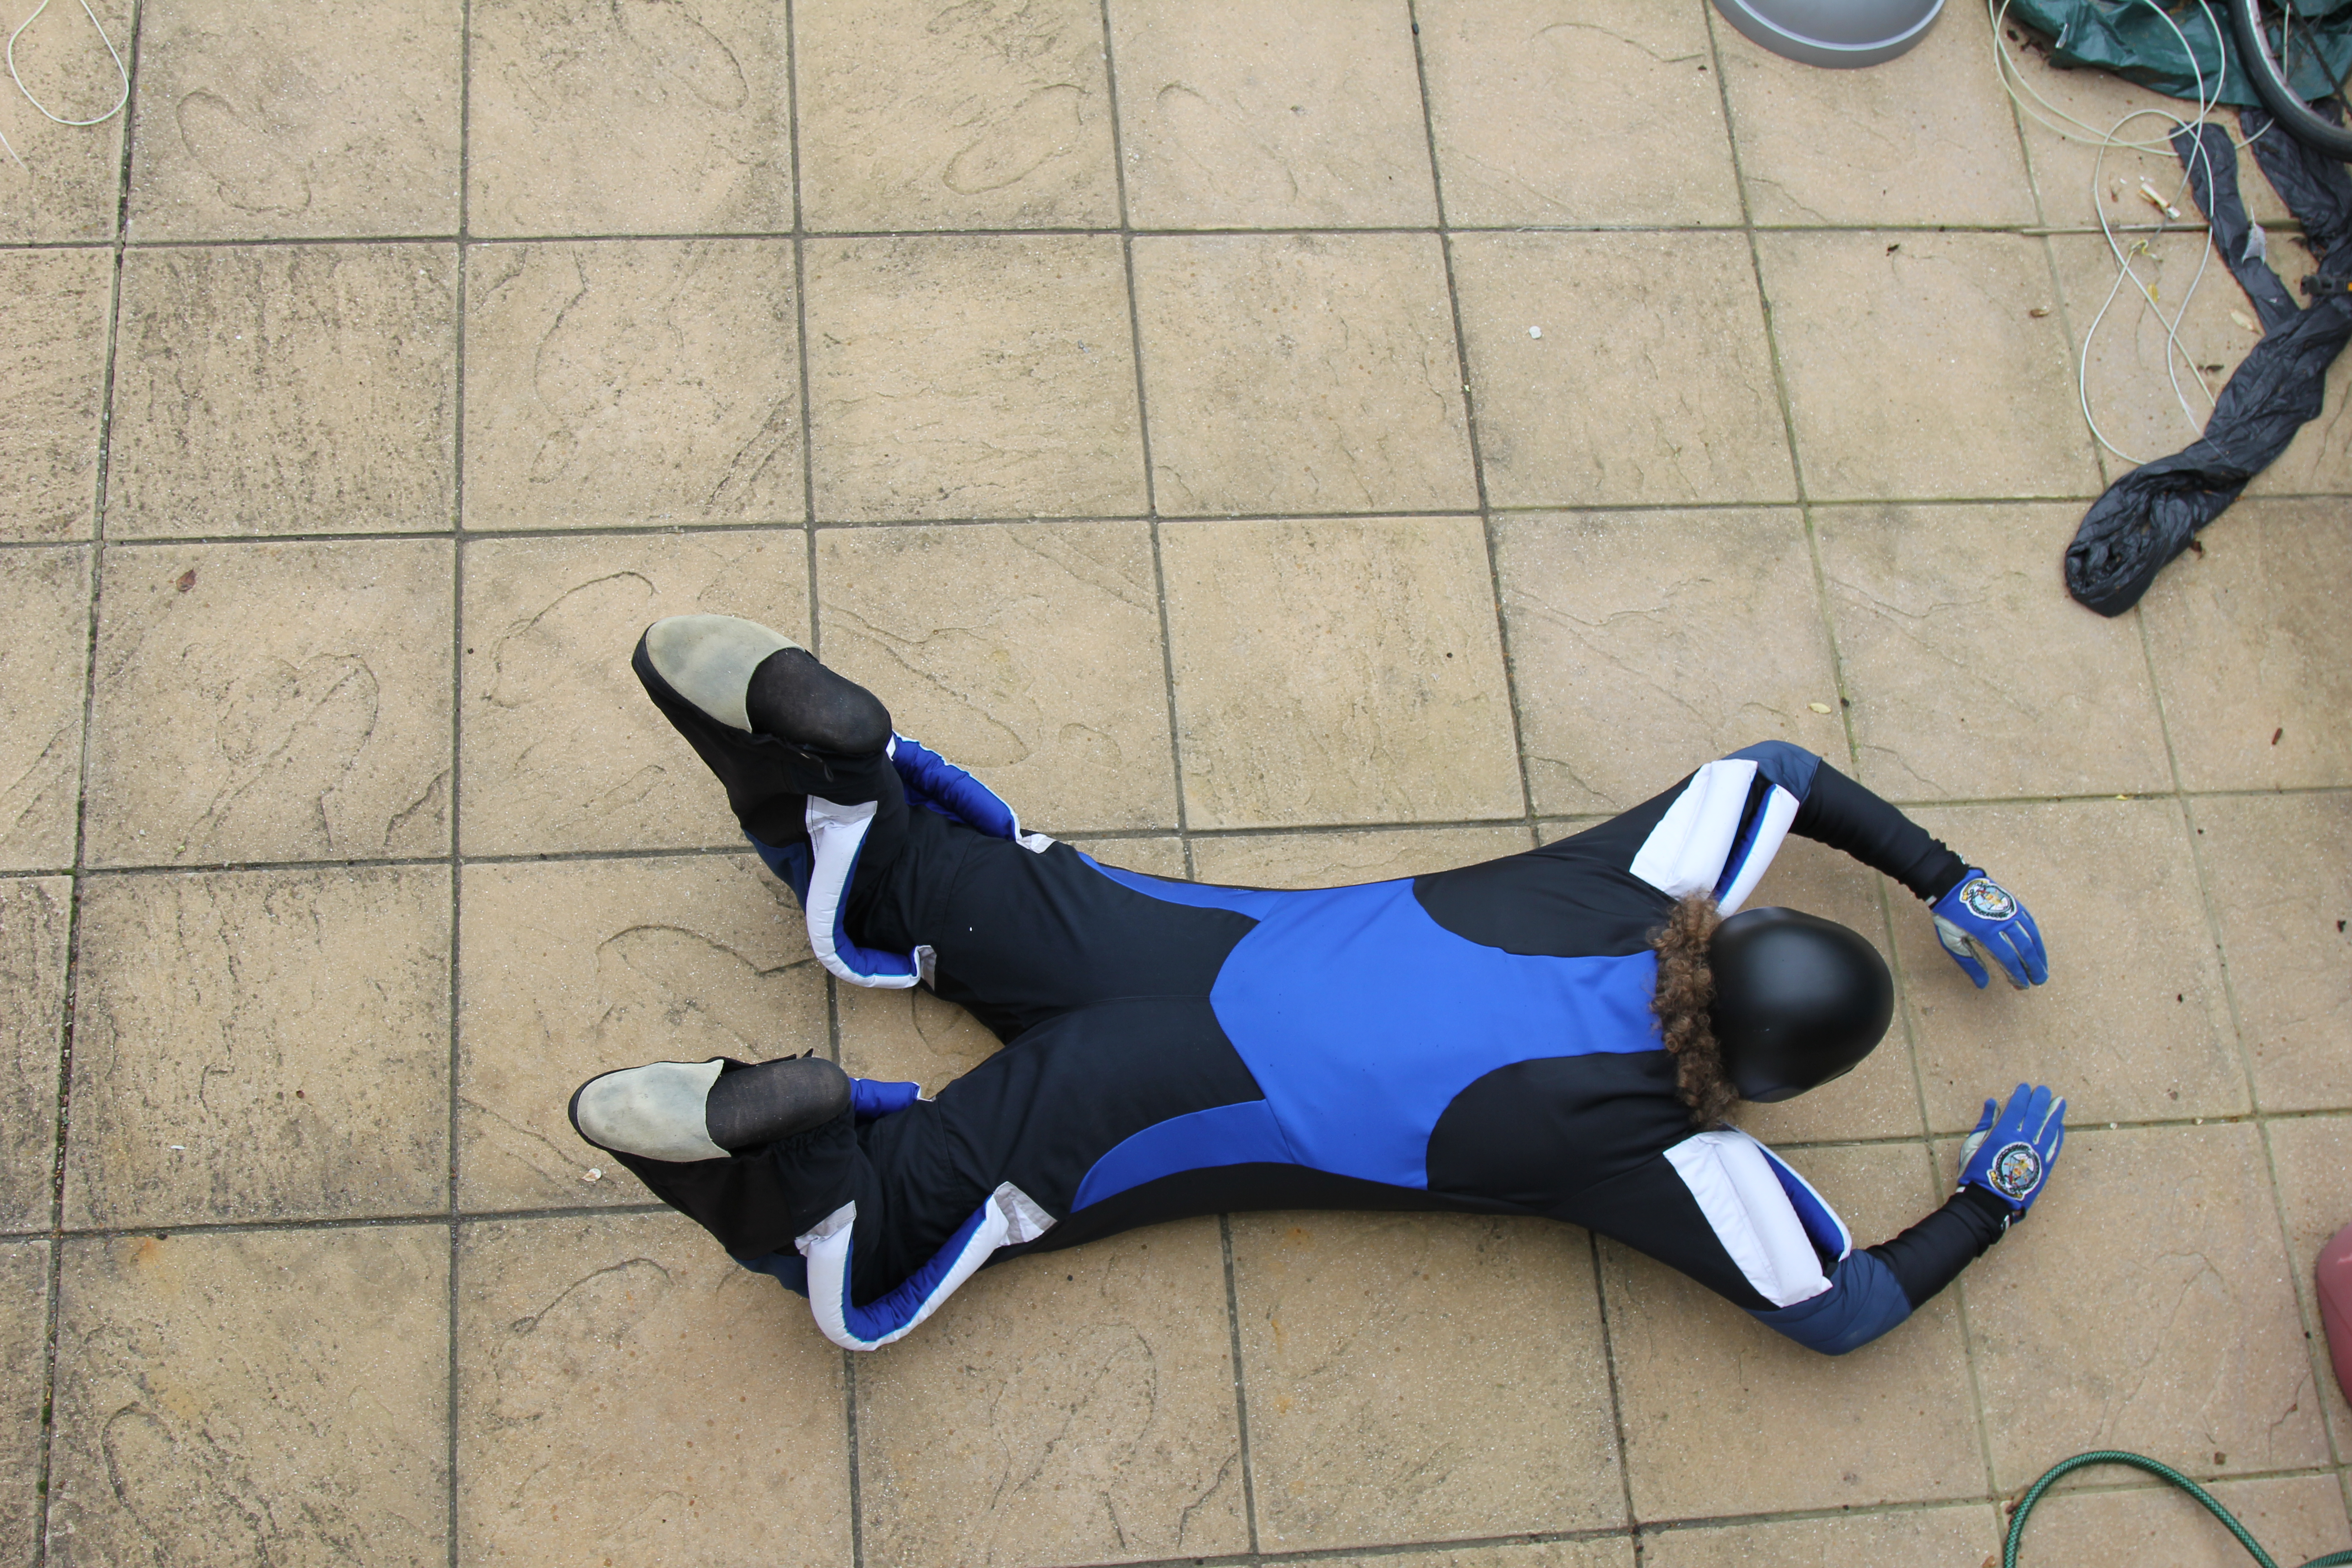
\includegraphics[width=.95\linewidth]{skel_src.jpg}
  		\caption{Skeletonisation source image.}
  		\label{fig:skel_src}
	\end{subfigure}%
	%
	\begin{subfigure}{.5\textwidth}
  		\centering
  		\includegraphics[width=.95\linewidth]{skel_src_mask.jpg}
  		\caption{Binary mask of source image.}
  		\label{fig:skel_src_mask}
	\end{subfigure}\\
	%
	\begin{subfigure}{\textwidth}
  		\centering
  		\includegraphics[width=\linewidth]{skel.jpg}
  		\caption{Result of skeletonisation function. Erroneous bifurcations are circled in red.}
  		\label{fig:skel}
	\end{subfigure}\\
	%
	\begin{subfigure}{\textwidth}
  		\centering
  		\includegraphics[width=\linewidth]{skel_reduced.jpg}
  		\caption{Result of skeleton simplification algorithm.}
  		\label{fig:skel_reduced}
	\end{subfigure}
\caption{Results of skeletonisation and simplification algorithms.}
\end{figure}
%
\subsubsection{Background Subtraction}
	A background subtraction algorithm has been implemented using the OpenCV libraries\cite{OpenCV}. However, this cannot be properly tested, as the stock wind tunnel footage currently being used is too noisy.
\section{Project Management}
In order to properly manage the project, weekly meetings are conducted between the student and supervisor; progress and possible next steps are discussed.\\
An initial Gantt chart was created in order to aid in time management \textbf{\emph{(see appendix A)}}. However, as the project progressed this Gantt chart was seen to be irrelevant and A new chart was produced \textbf{\emph{(see appendix B)}}.
	\subsection{Risk Management}
	A risk assessment was carried out in order to assess potential problems, and how they could be prevented/ resolved.
%
\begin{table}[H]
\centering
\resizebox{\columnwidth}{!}{%
\begin{tabular}{|l|l|l|l|l|}
\hline
\textbf{\begin{tabular}[c]{@{}l@{}}Potential\\   Problem\end{tabular}}                                                                     & \textbf{Loss (1-5)} & \textbf{\begin{tabular}[c]{@{}l@{}}Probibility\\   (1-5)\end{tabular}} & \textbf{Risk} & \textbf{Plan}                                                                                                                                                                             \\ \hline
\begin{tabular}[c]{@{}l@{}}Unable to get suitable\\ stock FS footage\end{tabular}                                                          & 4                   & 3                                                                      & 12            & \begin{tabular}[c]{@{}l@{}}Contact FS coaches to\\ ask for stock footage.\\ If this is not possible, record\\ a training session in the wind\\ tunnel with my 4-way FS team.\end{tabular} \\ \hline
\begin{tabular}[c]{@{}l@{}}Source code lost due to \\ home computer failure\end{tabular}                                                   & 5                   & 1                                                                      & 5             & \begin{tabular}[c]{@{}l@{}}All source code and project\\ documentation is backed up\\ on a private github repository.\end{tabular}                                                        \\ \hline
Severe Illness                                                                                                                             & 4                   & 1                                                                      & 4             & \begin{tabular}[c]{@{}l@{}}Time is factored into the initial\\ Gantt chart in order to account\\ for unforeseen problems,\\ such as illness.\end{tabular}                                 \\ \hline
\begin{tabular}[c]{@{}l@{}}Creating an active shape model\\ is more difficult and time \\ consuming than expected\end{tabular}             & 4                   & 3                                                                      & 12            & \begin{tabular}[c]{@{}l@{}}More time can be contributed\\ to the project, should this be\\ the case.\end{tabular}                                                                         \\ \hline
\begin{tabular}[c]{@{}l@{}}Fitting a stick man model to a\\ skeleton is more difficult and \\ time consuming than expected\end{tabular}    & 4                   & 3                                                                      & 12            & \begin{tabular}[c]{@{}l@{}}More time can be contributed\\ to the project, should this be\\ the case.\end{tabular}                                                                         \\ \hline
\begin{tabular}[c]{@{}l@{}}No project work is completed \\ during the exam period, and the\\   project falls behind schedule\end{tabular} & 3                   & 4                                                                      & 12            & \begin{tabular}[c]{@{}l@{}}After the exam period, extra\\time can be contributed to\\the project.\end{tabular}                                                                          \\ \hline
\end{tabular}%
}
\end{table}
%
\end{document}